\documentclass[12pt,a4paper]{article}
\usepackage[utf8]{inputenc}
\usepackage{graphicx}   % Para insertar gráficos
\usepackage{geometry}   % Para márgenes
\geometry{top=2.5cm, bottom=2.5cm, left=2.5cm, right=2.5cm}
\usepackage{setspace}   % Para controlar espacio entre líneas
\usepackage{lipsum}     % Solo para texto de ejemplo
\renewcommand{\contentsname}{Contenidos}

% ---------------- Caratula ----------------
\begin{document}
\begin{titlepage}
    \centering
    \vspace*{2cm}
    
    {\Huge \textbf{Alix Partners: La Casa de Asterión}}\\[0.5cm]
    {\Large Predicción de demanda y optimización de precios}\\[1.5cm]
    
    {\Large 2025}\\[2cm]

\end{titlepage}

% ---------------- Contenido ----------------
\tableofcontents
\newpage

\section{Introducción}

En esta competencia, nos fue dado el siguiente desafío: un negocio de ventas minoristas, llamado "La Casa de Asterión", ha sufrido una reducción de ganancias 
en el último tiempo, y necesita mejorar su estrategia de precios para solucionar este problema. La empresa ha proporcionado los siguientes datos: las transacciones 
de ventas de los últimos 3 años, especificando las tiendas, los productos vendidos y sus precios. Además, también contamos con datos sobre las tiendas, como su ubicación, 
y sobre los productos, como su categoría y marca. 

\vspace{0.2cm}

Entonces, valiéndonos de toda esta información, nuestro objetivo es contruir un modelo capaz de predecir la demanda diaria de los prodcutos de la próxima semana a 
partir del precio y otras variables, y con el mismo, optimizar los precios para maximizar las ganancias.

\vspace{0.2cm}

Dado que desconocemos si el cliente tiene conocimientos técnicos acerca de programación y desarrollo de modelos de AI, 
hemos decidido dividir este informe en dos secciones: por un lado, un análisis económico, el cual no necesita conocimientos técnicos para ser entendido, 
donde realizamos un análisis de datos básico y exponemos una estrategia de precios que, según las predicciones hechas, debería aumentar las ganancias; 
y por otro lado, realizamos un análisis técnico, en donde detallamos el preprocesamiento de datos, la construcción y entrenamiento del modelo predictivo 
y la metodología de optimización de precios.

\vspace{0.2cm}

Además, todo el código fuente utilizado para el trabajo está disponible adjunto al informe.



\newpage

\section{Análisis Económico}

En primer lugar, nos preguntamos por qué se ha producido una caída de las ganancias y qué tan grave es. Para esto, se puede observar 
en el siguiente gráfico cómo fue evolucionando la ganancia total de la empresa a lo largo del tiempo, y cómo la misma ha ido disminuyendo de a poco 
en el transcurso del tiempo.

\begin{center}
    \makebox[\textwidth][c]{%
        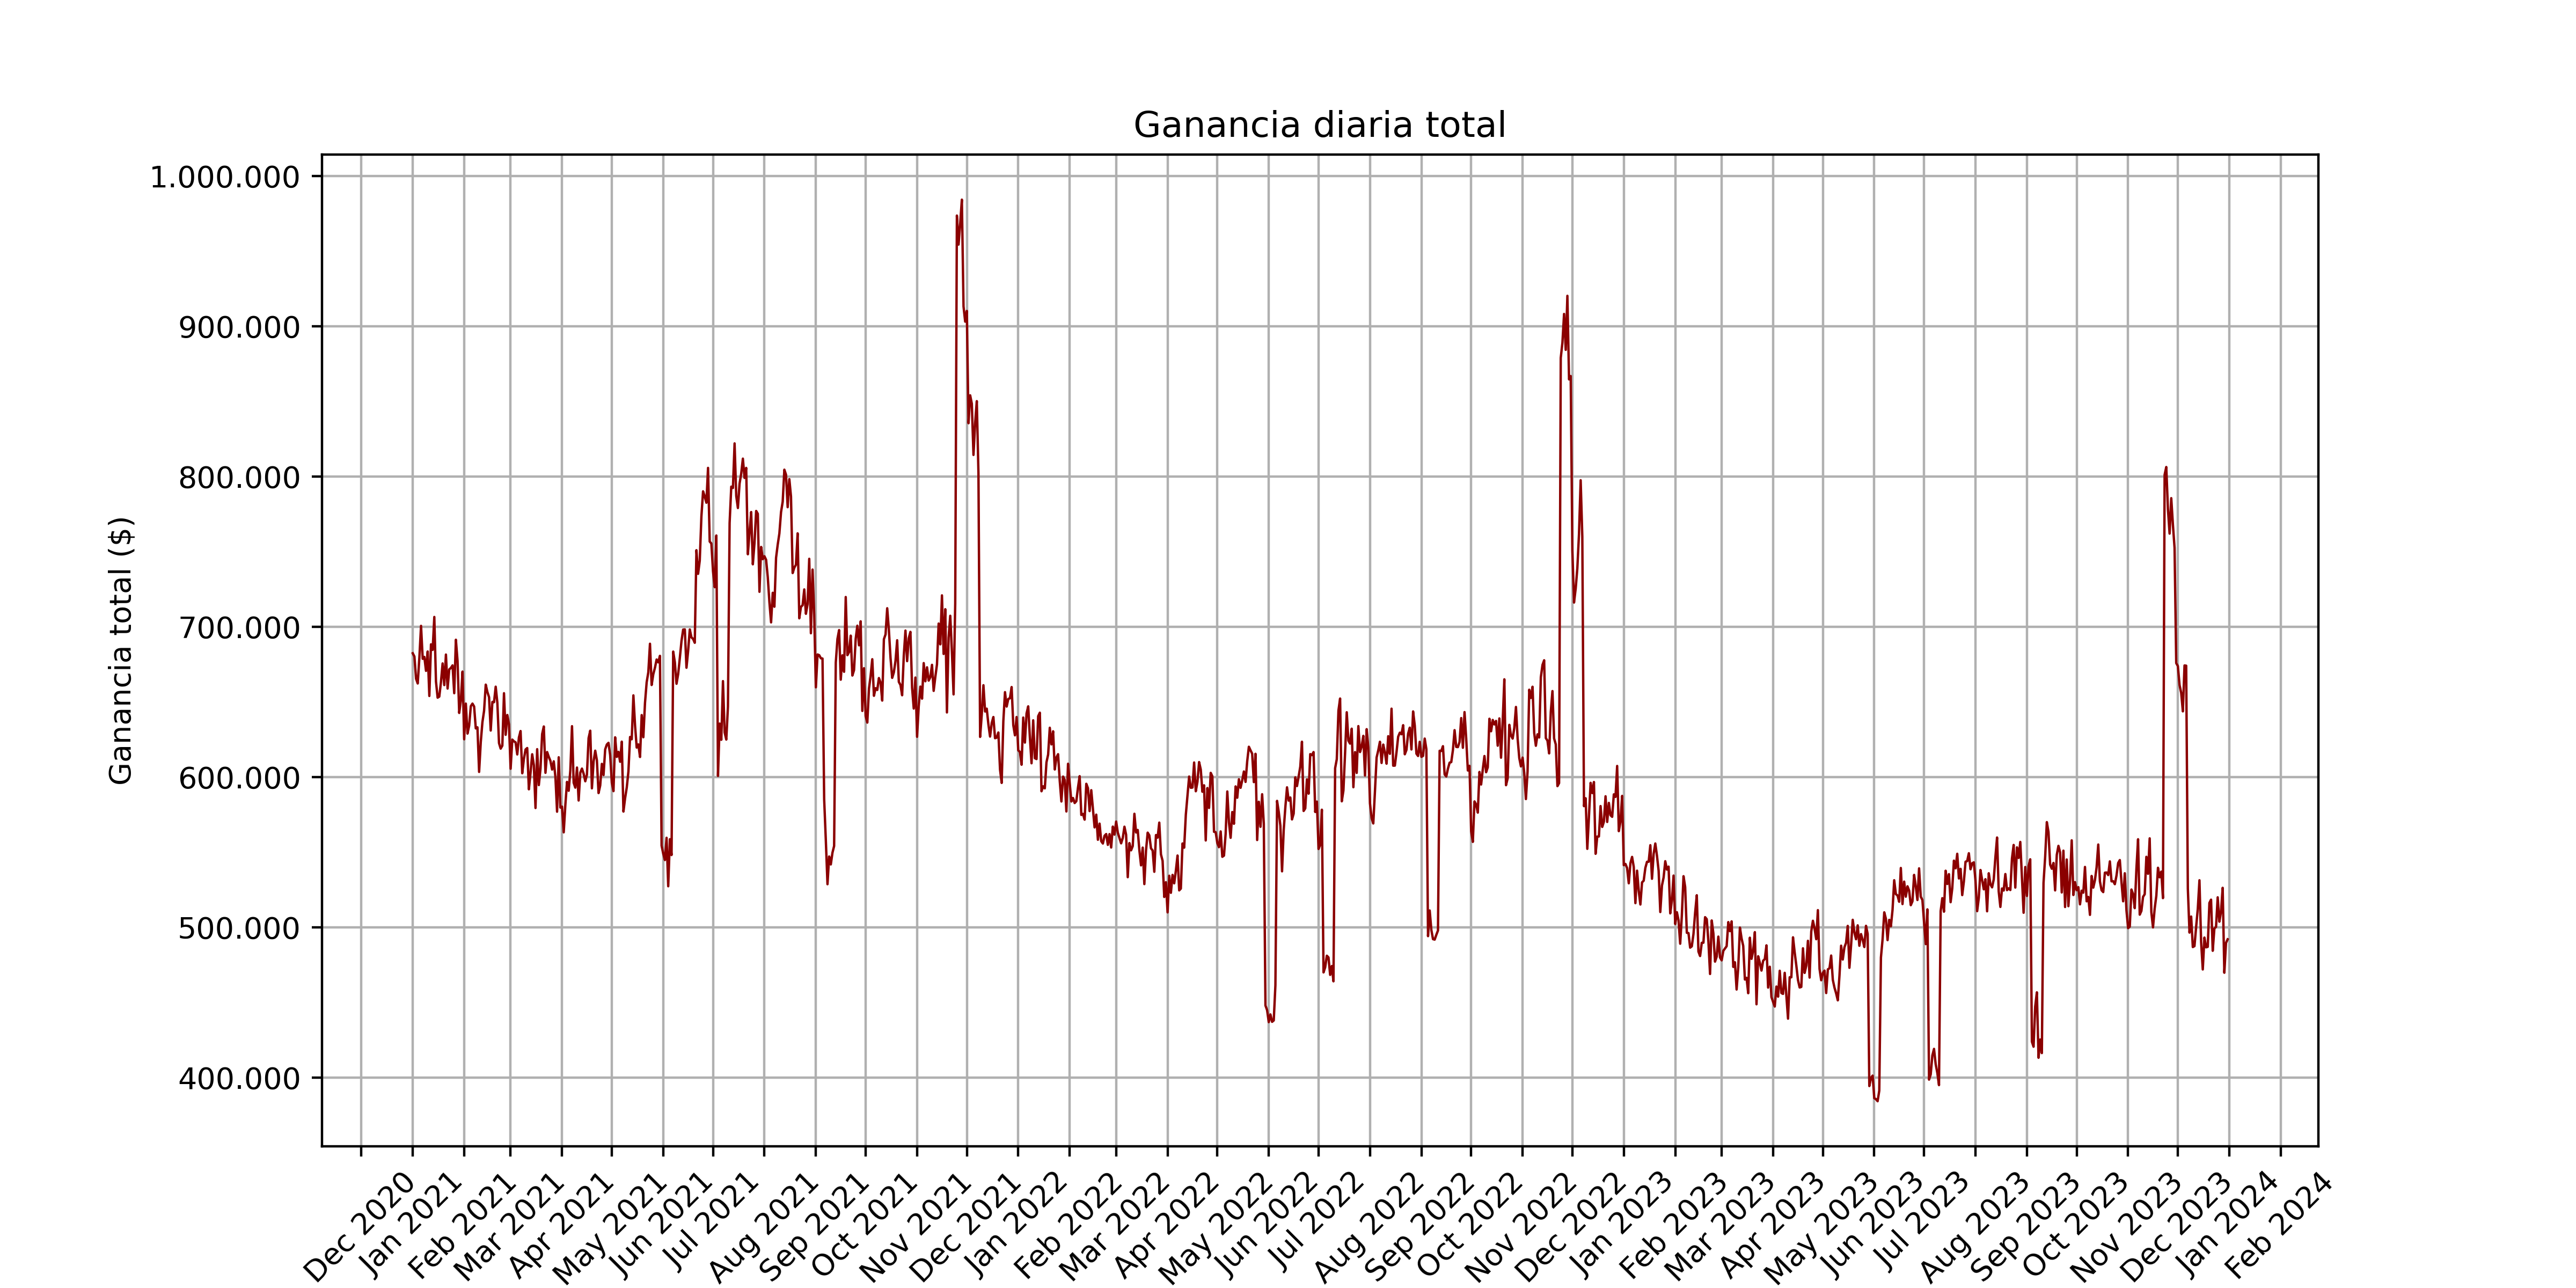
\includegraphics[width=1.2\textwidth]{graficos/ganancia_diaria_total.png}%
    }
\end{center}

En concreto, con respecto al primer año, las ganancias totales se han reducido un 11.3\% en el segundo año y un 23.7\% en el tercer año, 
lo cual puede resultar preocupante.

\vspace{0.2cm}

Este fenómeno puede deberse en gran parte a la reducción de la demanda total, que ha disminuído 10\% el primer año y un 21.2\% en el segundo año. 
Esto se puede apreciar en el siguiente gráfico, además de cómo varía la demanda según la categoría de los productos:

\begin{center}
    \makebox[\textwidth][c]{%
        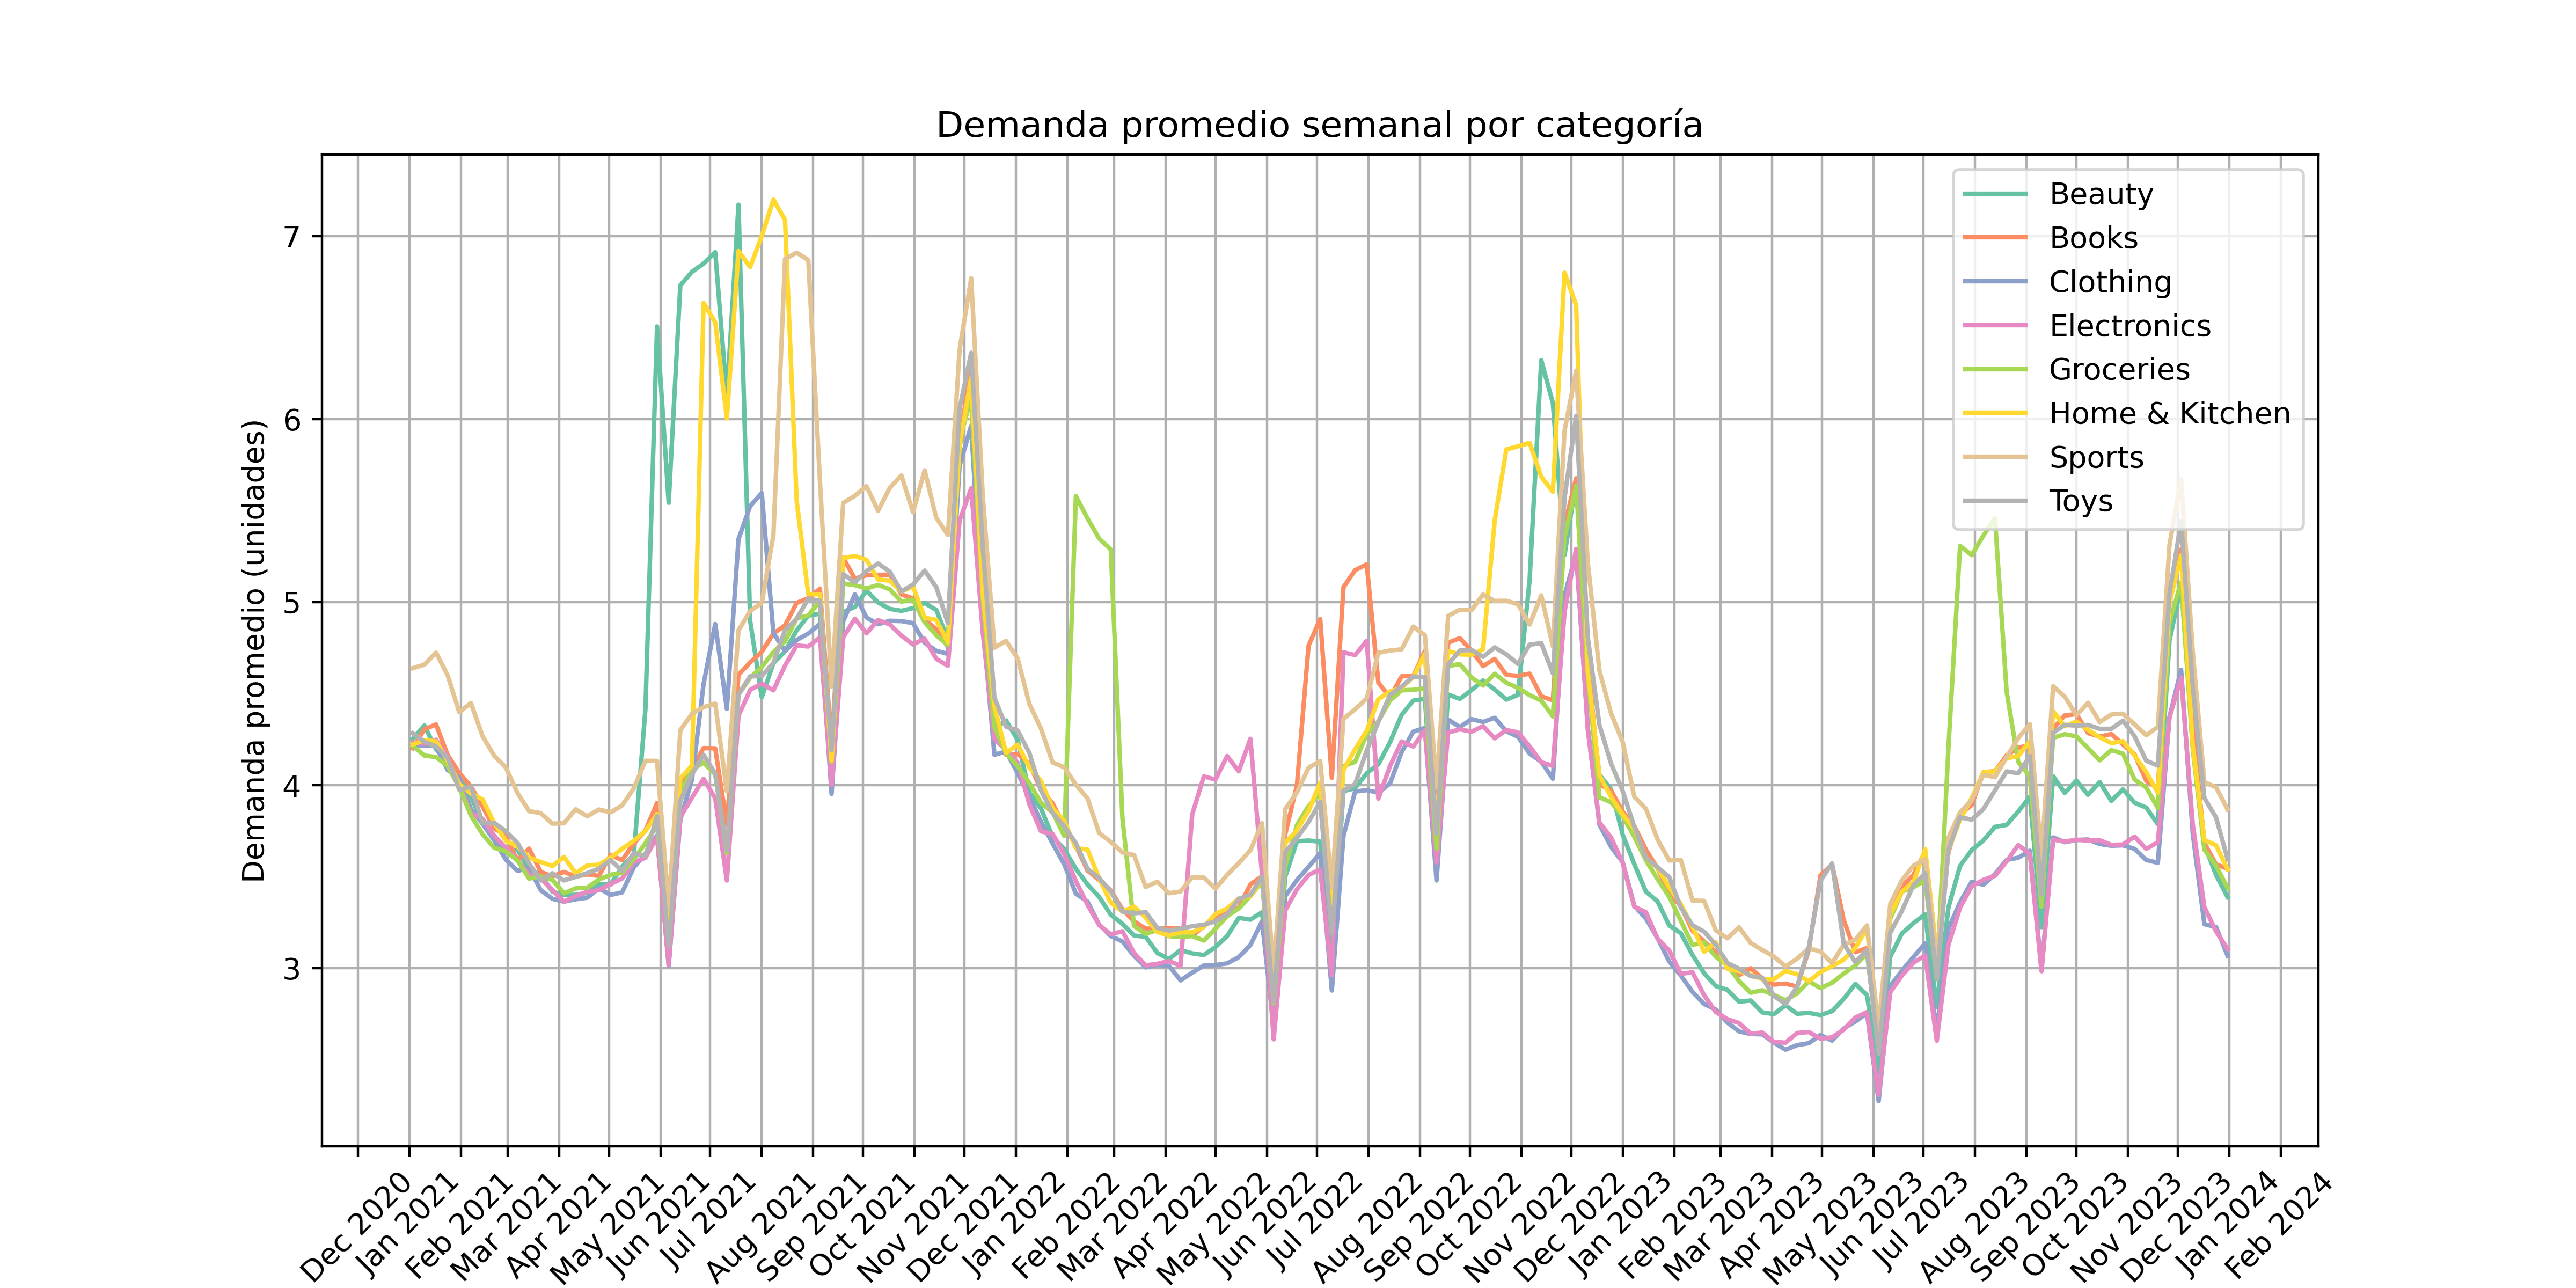
\includegraphics[width=1.2\textwidth]{graficos/demanda_promedio_semanal_por_categoria.png}%
    }
\end{center}

Al comparar este último gráfico con el de las ganancias totales, se pueden observar 3 comportamientos similares: 
\begin{itemize}
    \item A nivel global, hay una reducción gradual de las ganancias y la demanda 
    \item En cada año, en general hay un incremento a medida que transcurre el año y un descenso a principios de cada año.
    \item En Mayo, Junio y Agosto hay caídas abruptas, mientras que en Diciembre hay un incremento sustancial, seguramente debido a las festividades.
\end{itemize}

Decidimos analizar si estos descensos en la demanda se debían a cambios en los precios, sin embargo, en el siguiente gráfico se aprecia 
que en promedio los precios han seguido un mismo patrón:

\begin{center}
    \makebox[\textwidth][c]{%
        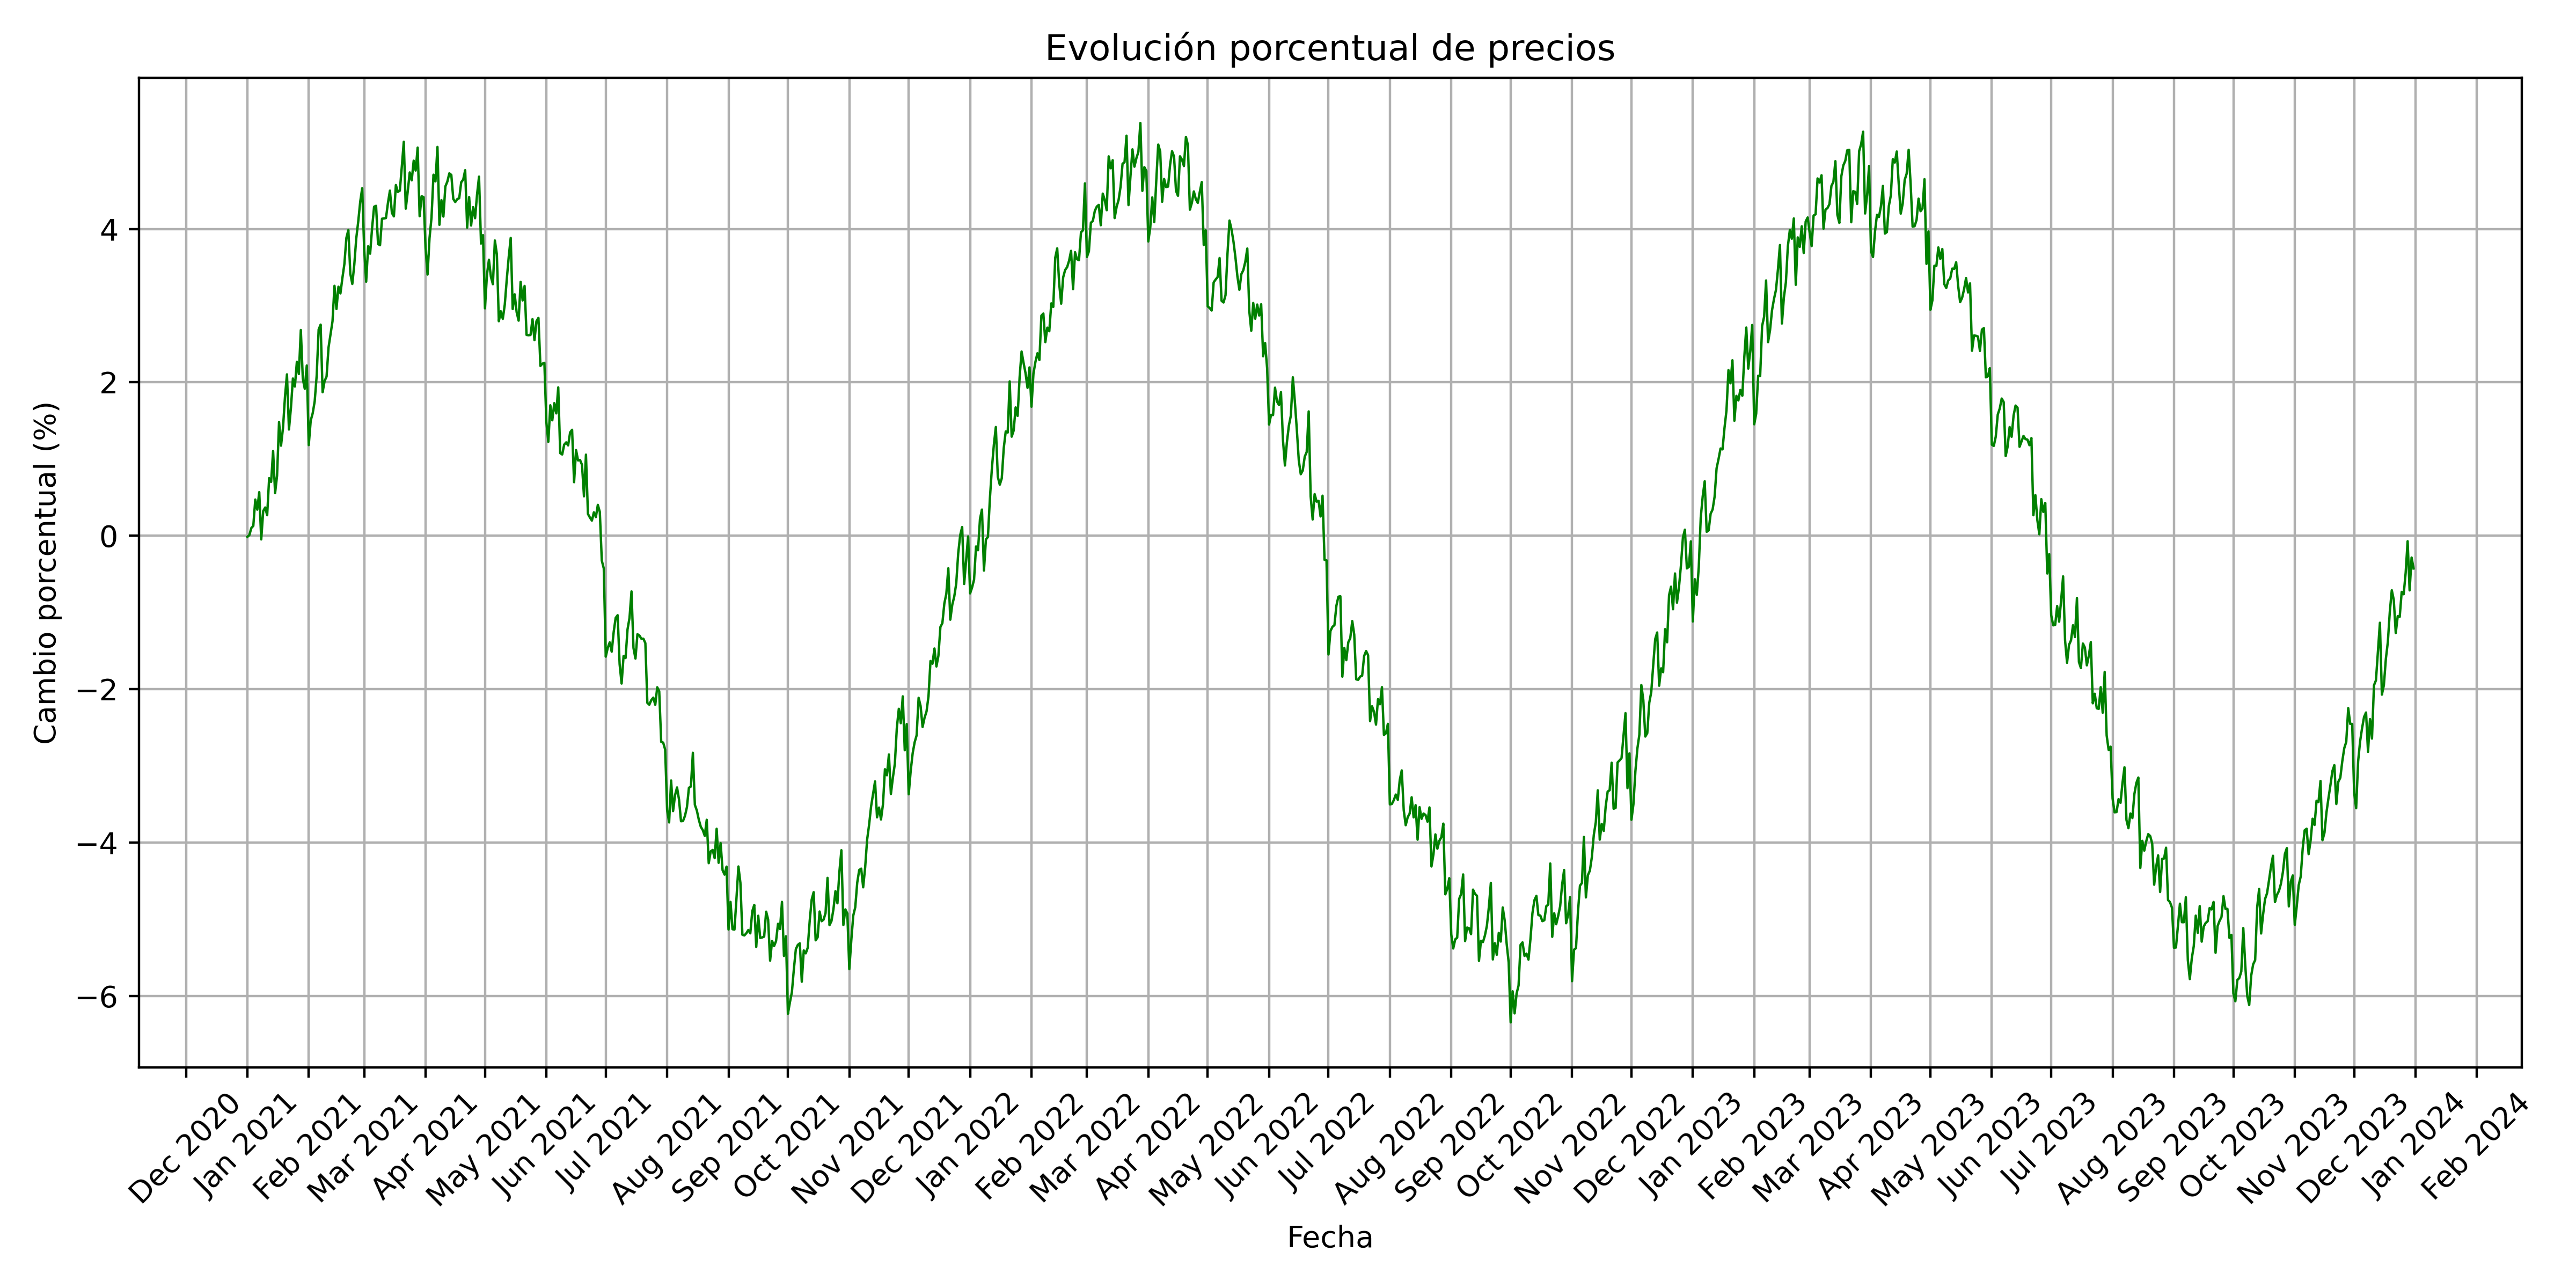
\includegraphics[width=1\textwidth]{graficos/evolucion_porcentual_precios.png}%
    }
\end{center}

Dado que los precios en general no han variado pero la demanda sí, nos lleva a pensar que es posible que un factor 
importante en la reducción sea la estrategia de precios actual, la cual no aprovecha correctamente 
la estacionalidad de la demanda. De hecho, en cada uno de los productos podemos 
observar un comportamiento similar: los precios oscilan de manera periódica a lo largo del año, pero en ciertos 
momentos, hay caídas abruptas en los precios, como se muestra a continuación.

\begin{center}
    \makebox[\textwidth][c]{%
        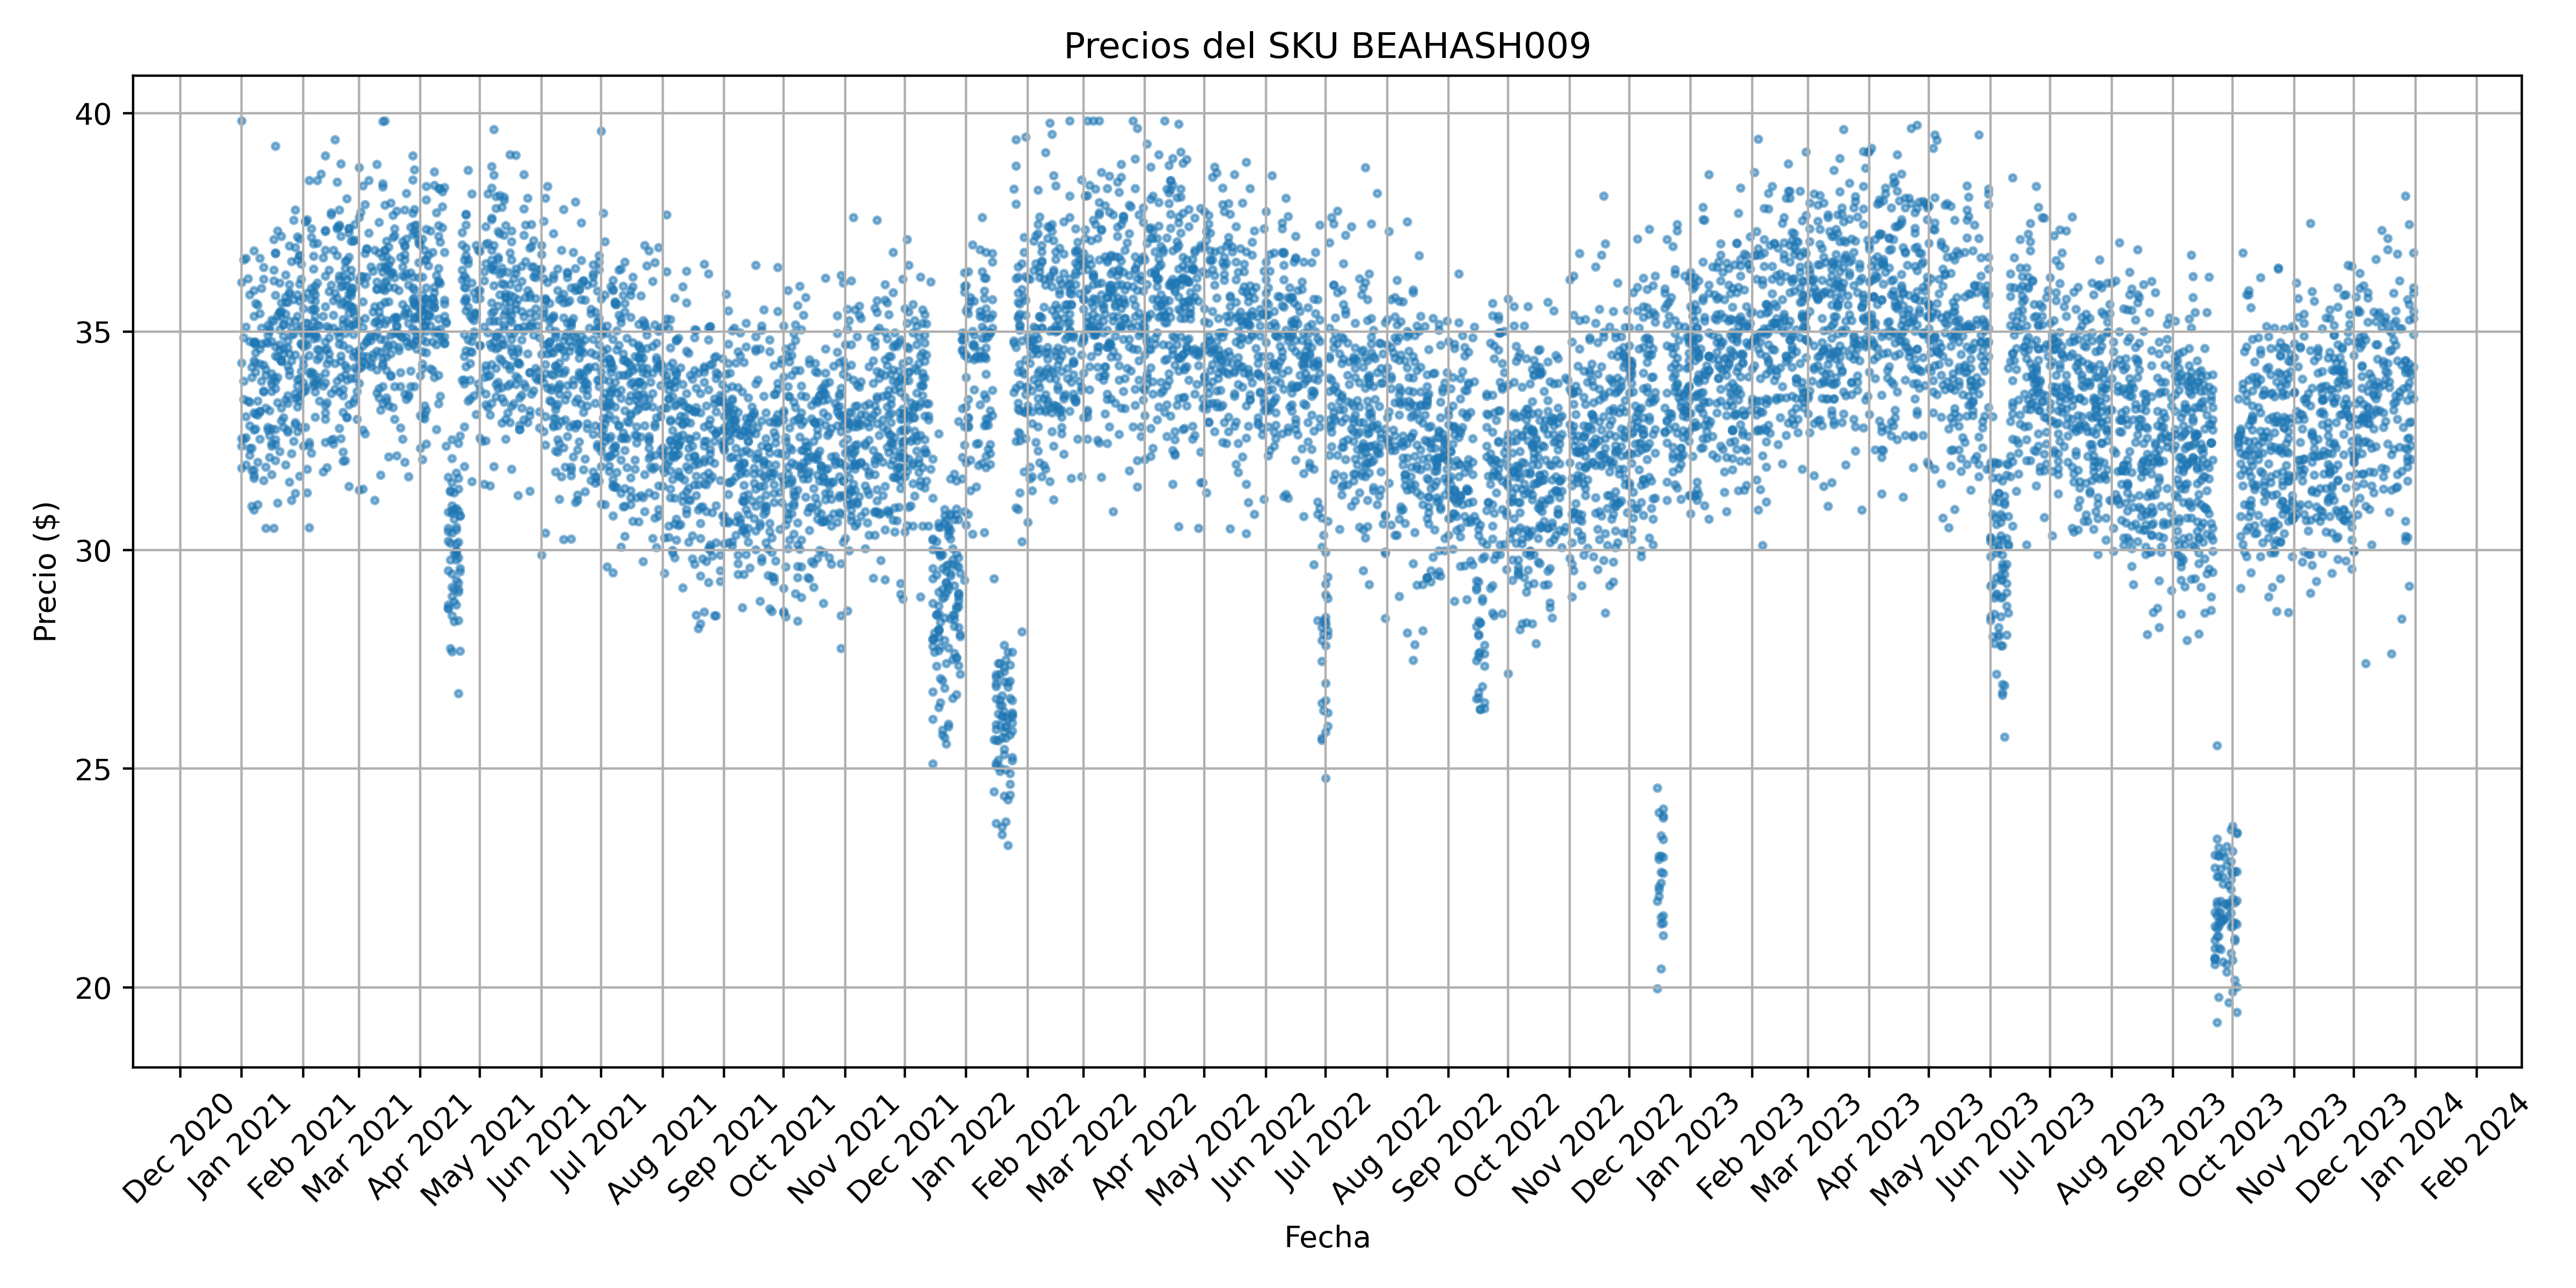
\includegraphics[width=1\textwidth]{graficos/precios_sku_BEAHASH009.png}%
    }
\end{center}

Por otro lado, la disminución de la demanda de diferentes productos no afecta a las ganancias de la misma 
manera, puesto que las ganancias están constituídas mayormente por productos de la categoría de electrónica:

\begin{center}
    \makebox[\textwidth][c]{%
        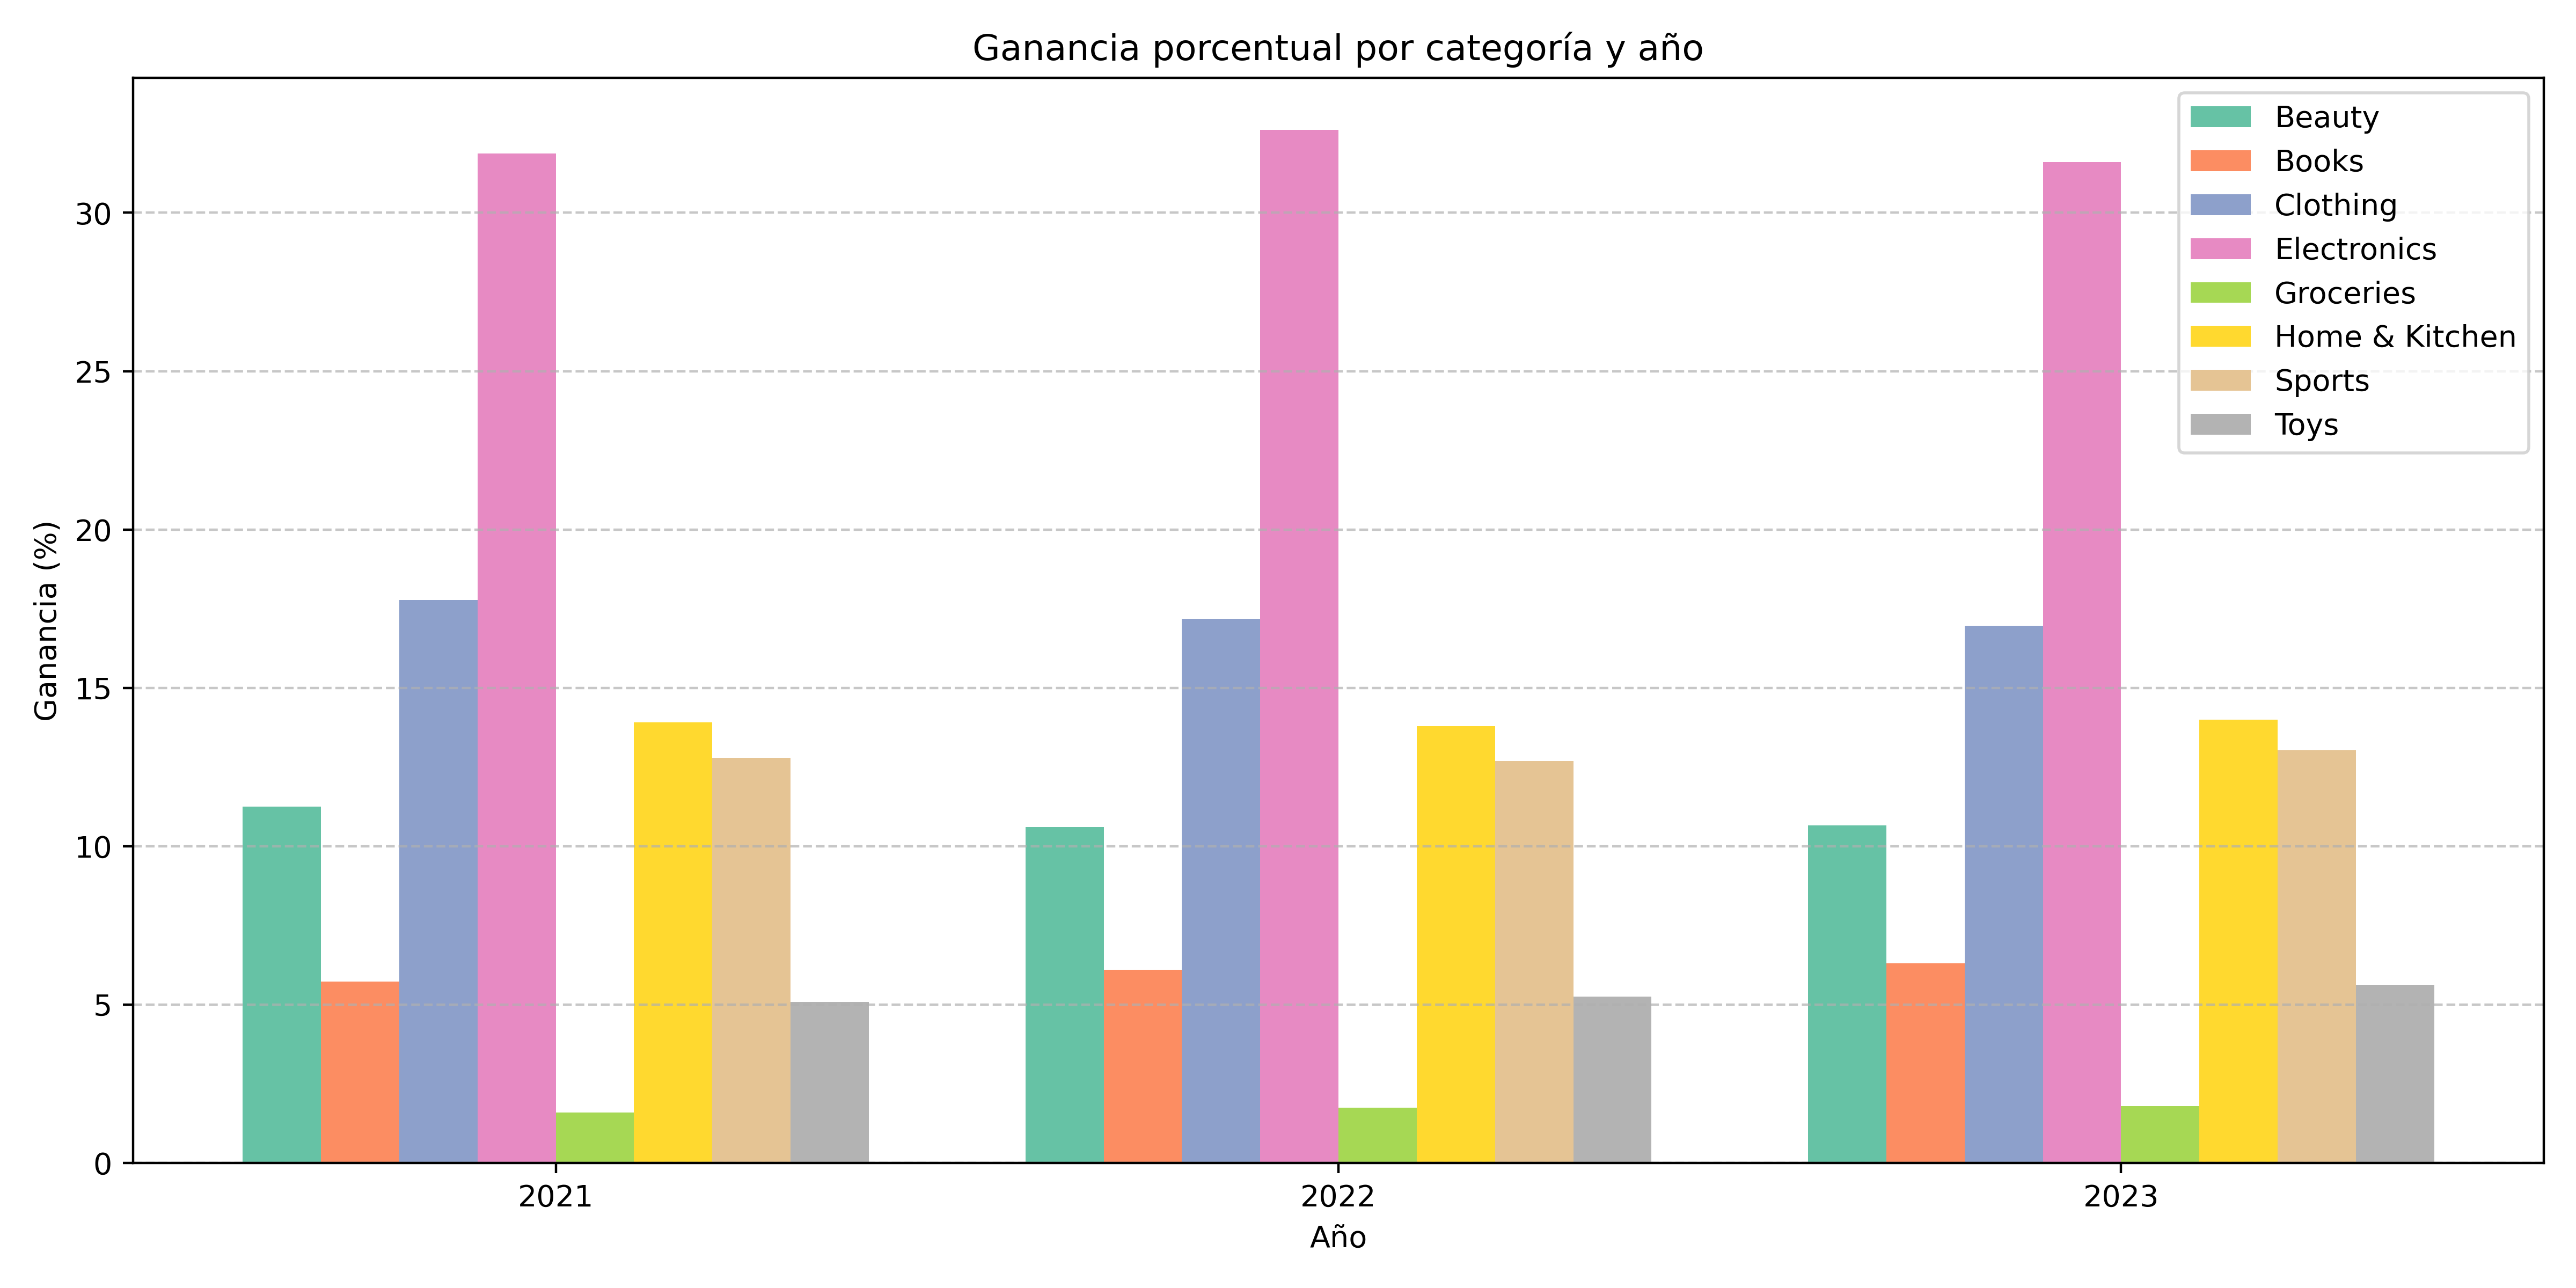
\includegraphics[width=1\textwidth]{graficos/ganancia_porcentual_por_categoria.png}%
    }
\end{center}

Antes de continuar, es importante aclarar que el subgrupo de productos de "Basketball" no registró ninguna venta en los últimos 3 años, lo que puede deberse 
a una falla en la carga de datos o a que el producto no se comercializa en las tiendas.

\vspace{0.2cm}

Teniendo en cuenta todo lo anterior, 










\newpage

\section{Análisis Técnico}

\subsection{Preprocesamiento de Datos}

Comenzamos el trabajo explorando los datos proporcionados y completando los datos faltantes. Después, nos quedamos con aquellas 
columnas que consideramos relevantes para el modelo e intentamos unir los 6 archivos csv en un mismo dataframe, sin embargo, 
los datos de los clientes no pudieron ser utilizados dado que las transacciones no contaban con el ID de cliente, por lo que no 
fue posible hacer unirlos. 

\vspace{0.2cm}

Entonces, nos quedamos con los siguientes datos para cada transacción: fecha, producto (SKU), tienda, 
precio, costo, cantidad vendida (en unidades y en total), categorías del producto y ubicación de la tienda, entre otros.

\vspace{0.2cm}

Por otro lado, descartamos ciertos outliers que consideramos que podían llegar a cesgar al modelo: transacciones con precios, 
cantidad vendida unitaria o cantidad vendida total fuera del 99.9\% quantile.



\subsection{Modelo Predictivo}

El modelo que mejores resultados nos proporcionó fue el LightGBM, el cual es un modelo de boosting que utiliza árboles de decisión y 
es capaz de manejas grandes volúmenes de datos de manera eficiente.

\vspace{0.2cm}

En primera instancia, utilizamos las transacciones dadas para entrenar el modelo, pero esto provocaba que después a la hora de 
predecir la demanda por producto y tienda, el modelo no tuviera en cuenta los días en que no hubo ventas y sobreestimara por mucho 
la demanda. Por lo tanto, decidimos crear un dataframe con todas las combinaciones posibles de fechas, productos y tiendas, y completar 
los días en que no hubo ventas con un valor 0 en la cantidad vendida total.

\vspace{0.2cm}

Además, a partir del dataframe completo, para que el modelo pueda entender mejor la estacionalidad de la demanda, 
creamos nuevos lagging features: agrupamos las transacciones por producto y calculamos 
una media móvil de la cantidad vendida total y su desviación estándar de los últimos días, para distintas ventanas temporales. 
Hicimos lo mismo pero agrupando por tienda, como también por subgrupo de productos.

\vspace{0.2cm}

Por otro lado, para que el modelo pueda relacionar mejor el precio y la demanda, creamos otros lagging features sobre los precios: 
agrupando las transacciones por producto, calculamos la media móvil y desviación estándar del cambio porcentual del precio de los 
últimos días, para distintas ventanas temporales. También hicimos lo mismo, pero agrupando por subgrupo de productos.

\vspace{0.2cm}

Entonces, con el dataframe completo y los features agregados, comenzamos a probar el modelo. Para esto, no podíamos emplear un cross-validation 
convencional, dado que los lagging features hubieran generado data leakage, por lo que decidimos hacer un walk-forward validation: 
entrenar el modelo con los datos del primer año, predecir la demanda de la próxima semana, guardar las predicciones y compararlas con 
las ventas reales, y luego sumar 30 días a los datos de entrenamiento y repetir el proceso. De esta manera, podemos evaluar la performance del 
modelo prediciendo la demanda de la próxima semana, tal como se haría si tuviéramos que hacerlo en tiempo real.

\vspace{0.2cm}

El fine-tuning del modelo se debió hacer de manera manual, puesto que el entrenamiento de cada modelo tenía un gran costo computacional 
y, por lo tanto, un Grid Search no era viable con los recursos disponibles.



\subsection{Optimización de Precios}

Después de validar el modelo, elegimos los hiperparámetros que mejor performance nos dieron y entrenamos el modelo con todos los datos 
disponibles. Luego, creamos un dataframe template con todas las combinaciones posibles de fechas, productos y tiendas de la próxima semana, 
exluyendo las tiendas que cerraron. 

\vspace{0.2cm}

Debido a que probar todas las configuraciones de precios posibles para predecir cuál maximiza las ventas totales era computacionalmente inviable, primero 
redujimos el espacio de búsqueda: para cada producto, quitamos los precios que se apartaban demasiado del rango de los últimos días. Tomando como ejemplo 
los precios de BEAHASH009, ya vistos anteriormente, podemos ver a continuación los precios filtrados:

\begin{center}
    \makebox[\textwidth][c]{%
        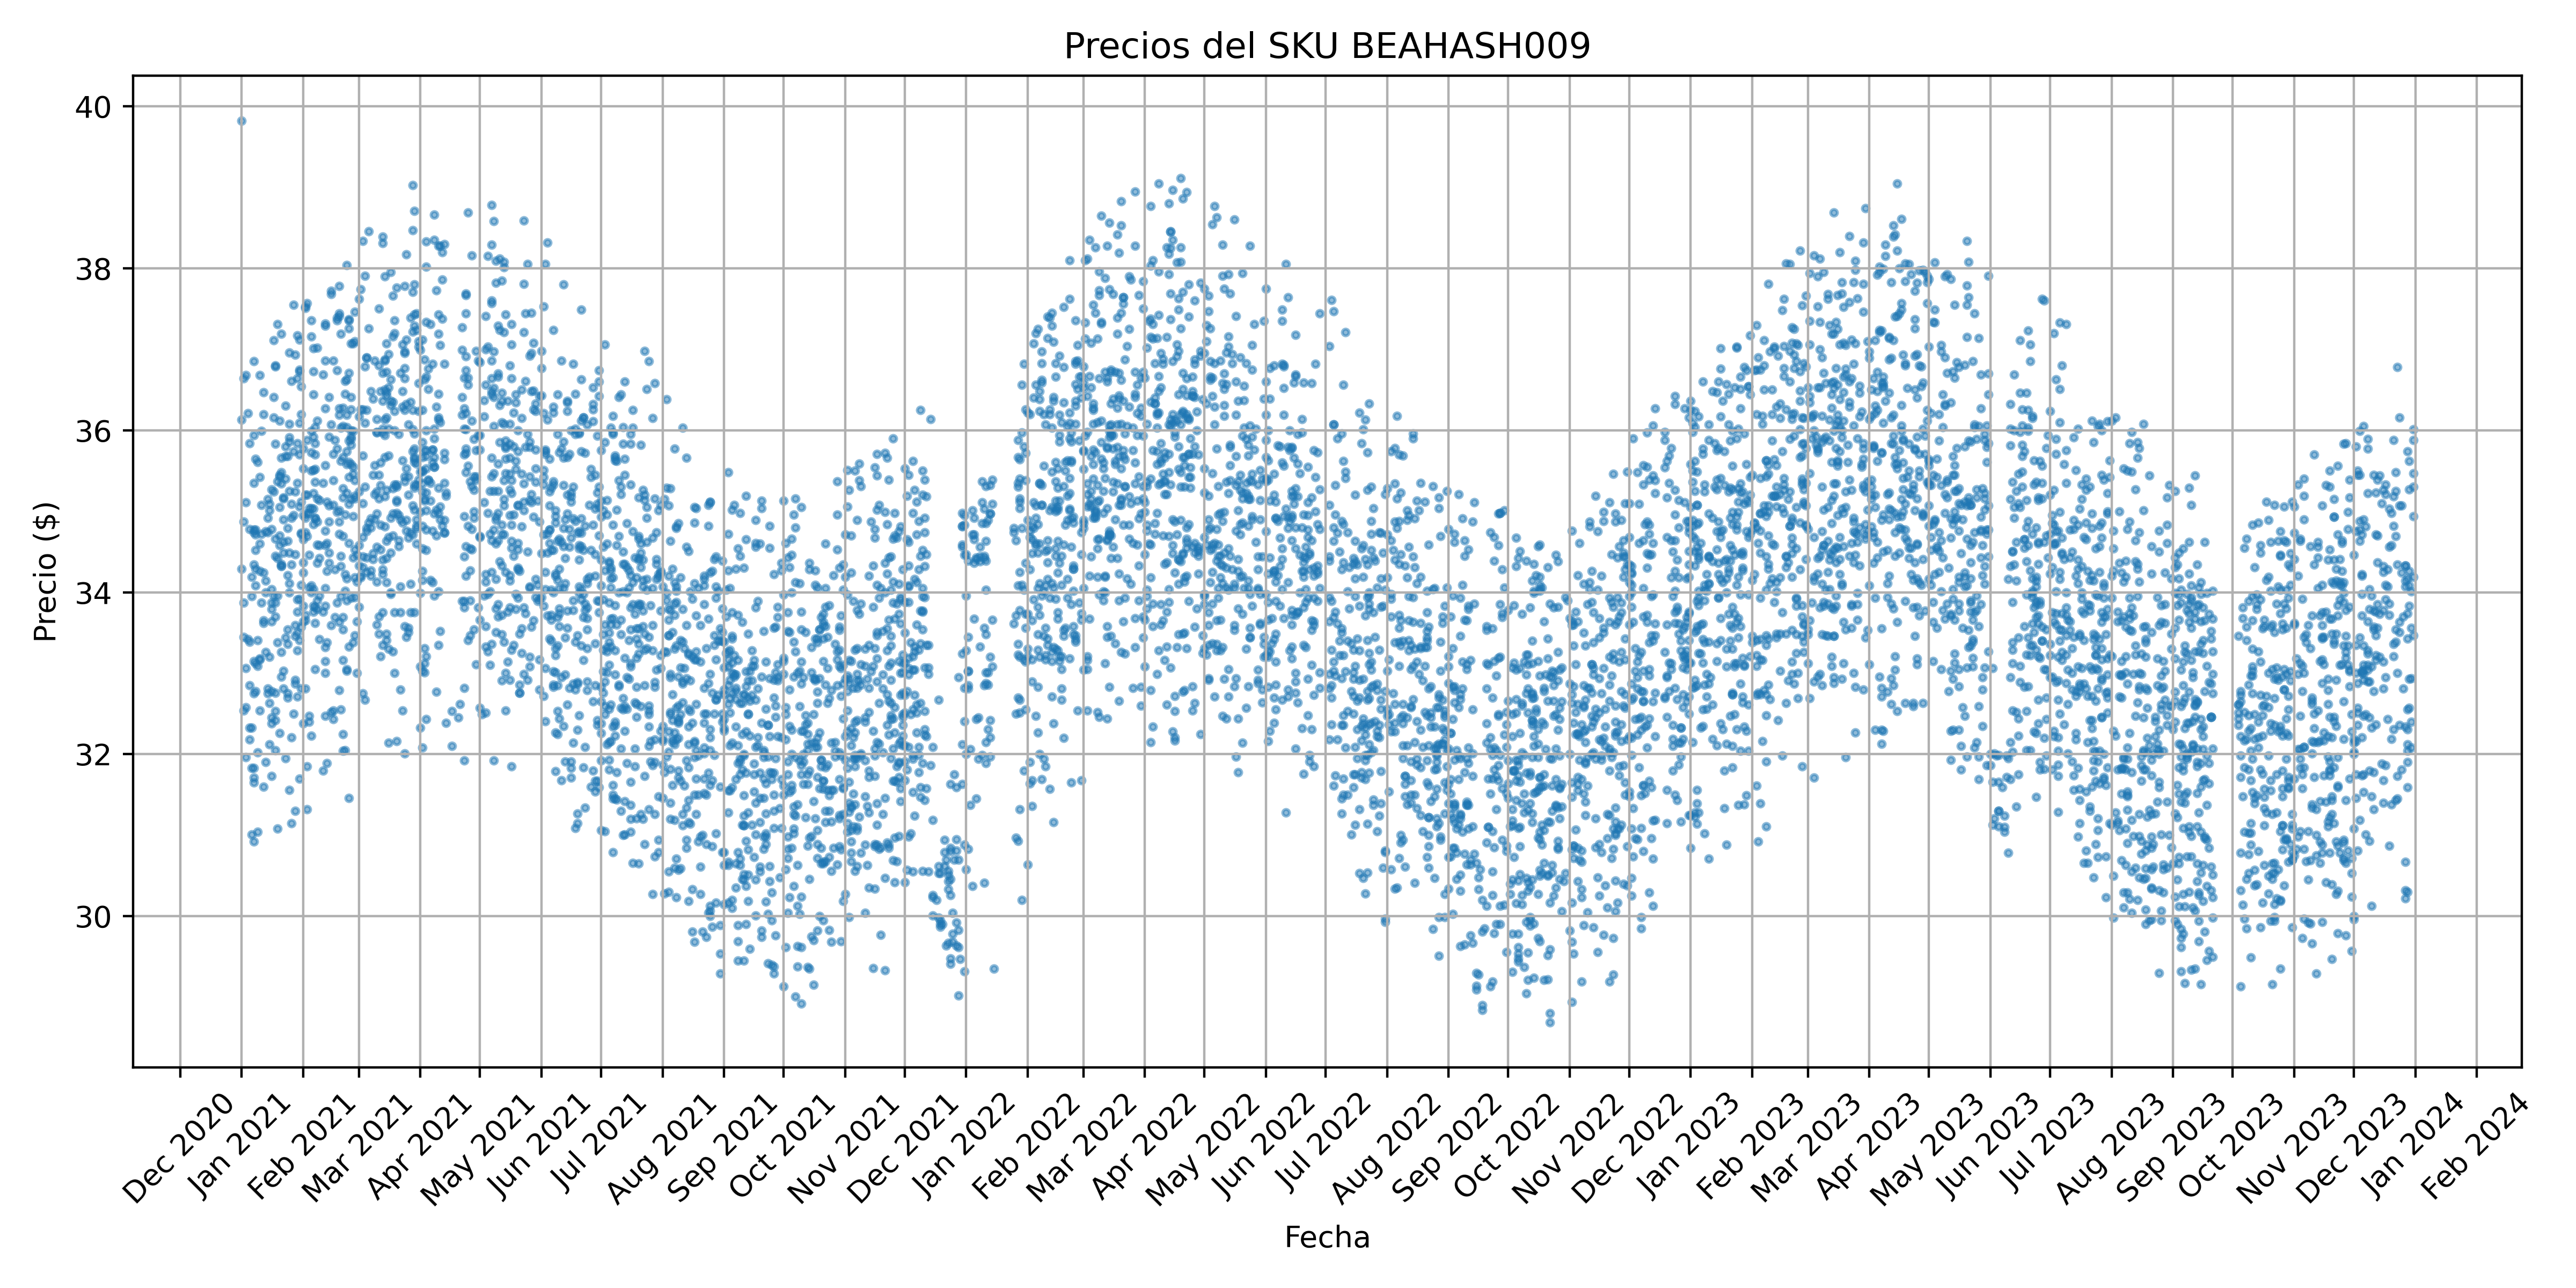
\includegraphics[width=1\textwidth]{graficos/precios_sku_BEAHASH009_filtrado.png}%
    }
\end{center}

Entonces, tomamos como rango de precios posibles para cada producto el máximo y el mínimo de los precios filtrados en los últimos 30 días. Cabe aclarar que 
aún así los datos con los precios no filtrados sí fueron utilizados para entrenar el modelo.

\vspace{0.2cm}

Además, para simplificar la implementación de la estrategia de precios, decidimos que los precios de los productos serán los mismos en todas las tiendas y 
para toda la semana.

\vspace{0.2cm}

Así, con un espacio de búsqueda más manejable, aplicamos una optimización bayesiana (con la librería Optuna) para encontrar la configuración de precios 
que maximiza las ganancias totales según las predicicones del modelo.



\newpage

\section{Consideraciones Finales}

\end{document}
